% Documento
\documentclass[12pt,a4paper,english,brazil]{article}
    
% Pacotes
\usepackage[utf8]{inputenc}
\usepackage[portuguese]{babel}
\usepackage[T1]{fontenc}
\usepackage[top=2cm,bottom=2cm,left=3cm,right=3cm]{geometry}
\usepackage{amsmath}
\usepackage{graphicx}           % para add imagens
\usepackage{xcolor}             % para usar \textcolor{}{}
\usepackage{float}              % para usar o [H] em imgs
\usepackage[num]{abntex2cite}   % padrão abnt para citação
\usepackage{indentfirst}        % indenta o 1º paragrafo 
\usepackage[colorlinks=true, allcolors=blue]{hyperref}

% Exercícios
\newtheorem{exer}{Exercício}

\begin{document}

% Título ------------------------------------------------------------
\title{ Exercício de Aplicação 3 \\ 
        SME 301 -  Métodos Numéricos para Engenharia I }
\date{\vspace{-5ex}}
\author{ Monitor João Paulo Casagrande Bertoldo \\
         Prof. Dr. Eduardo Fontoura Costa }
\maketitle
\vspace{15pt}

% Introdução --------------------------------------------------------
\section{Introdução}\label{sec-intro}

Dando continuidade ao Exercício de Aplicação 2, vamos analisar um detalhe no contexto do braço robótico de 3 graus de liberdade (GDL) visto anteriormente (Figura \ref{fig:robo}). \

No Exercício de Aplicação 2, desenvolvemos uma maneira de saber quais deveriam ser os ângulos dos motores para que a garra atingisse um ângulo desejado. 

\begin{figure}[H]
\centering
\includegraphics[width=0.7\textwidth]{roboFig.png}
\caption{\label{fig:robo}Desenho esquemático da geometria do robô.}
\end{figure}

Desta vez, falaremos um pouco sobre o aspecto dinâmico do robô, visto que, no exercício anterior, tratamos apenas da geometria do mesmo. \

Porém, nada dissemos a respeito de como fazer cada motor ter uma dada posição angular. Também não levamos em consideração o que acontece durante a transição de uma posição a outra. \

Portanto, a pergunta a ser respondida é a seguinte:

\begin{center} \begin{large}
\textbf{Dado um angulo desejado em um dos motores, qual comando deve ser a tensão de entrada e como o sistema se comporta durante a transição?}
\end{large} \end{center}

% Modelo ------------------------------------------------------------
\section{Modelo}\label{sec-modelo}

Por simplicidade, vamos tratar da dinâmica de apenas um braço isolado e seu acoplamento com um motor de corrente contínua ("motor CC" ou "motor DC"). Também vamos considerar que cada braço pode ser considerado como um barra de aço sólida de faces retangulares, como representado na Figura \ref{fig:motorEBraco}. \

\begin{figure}[H]
\centering
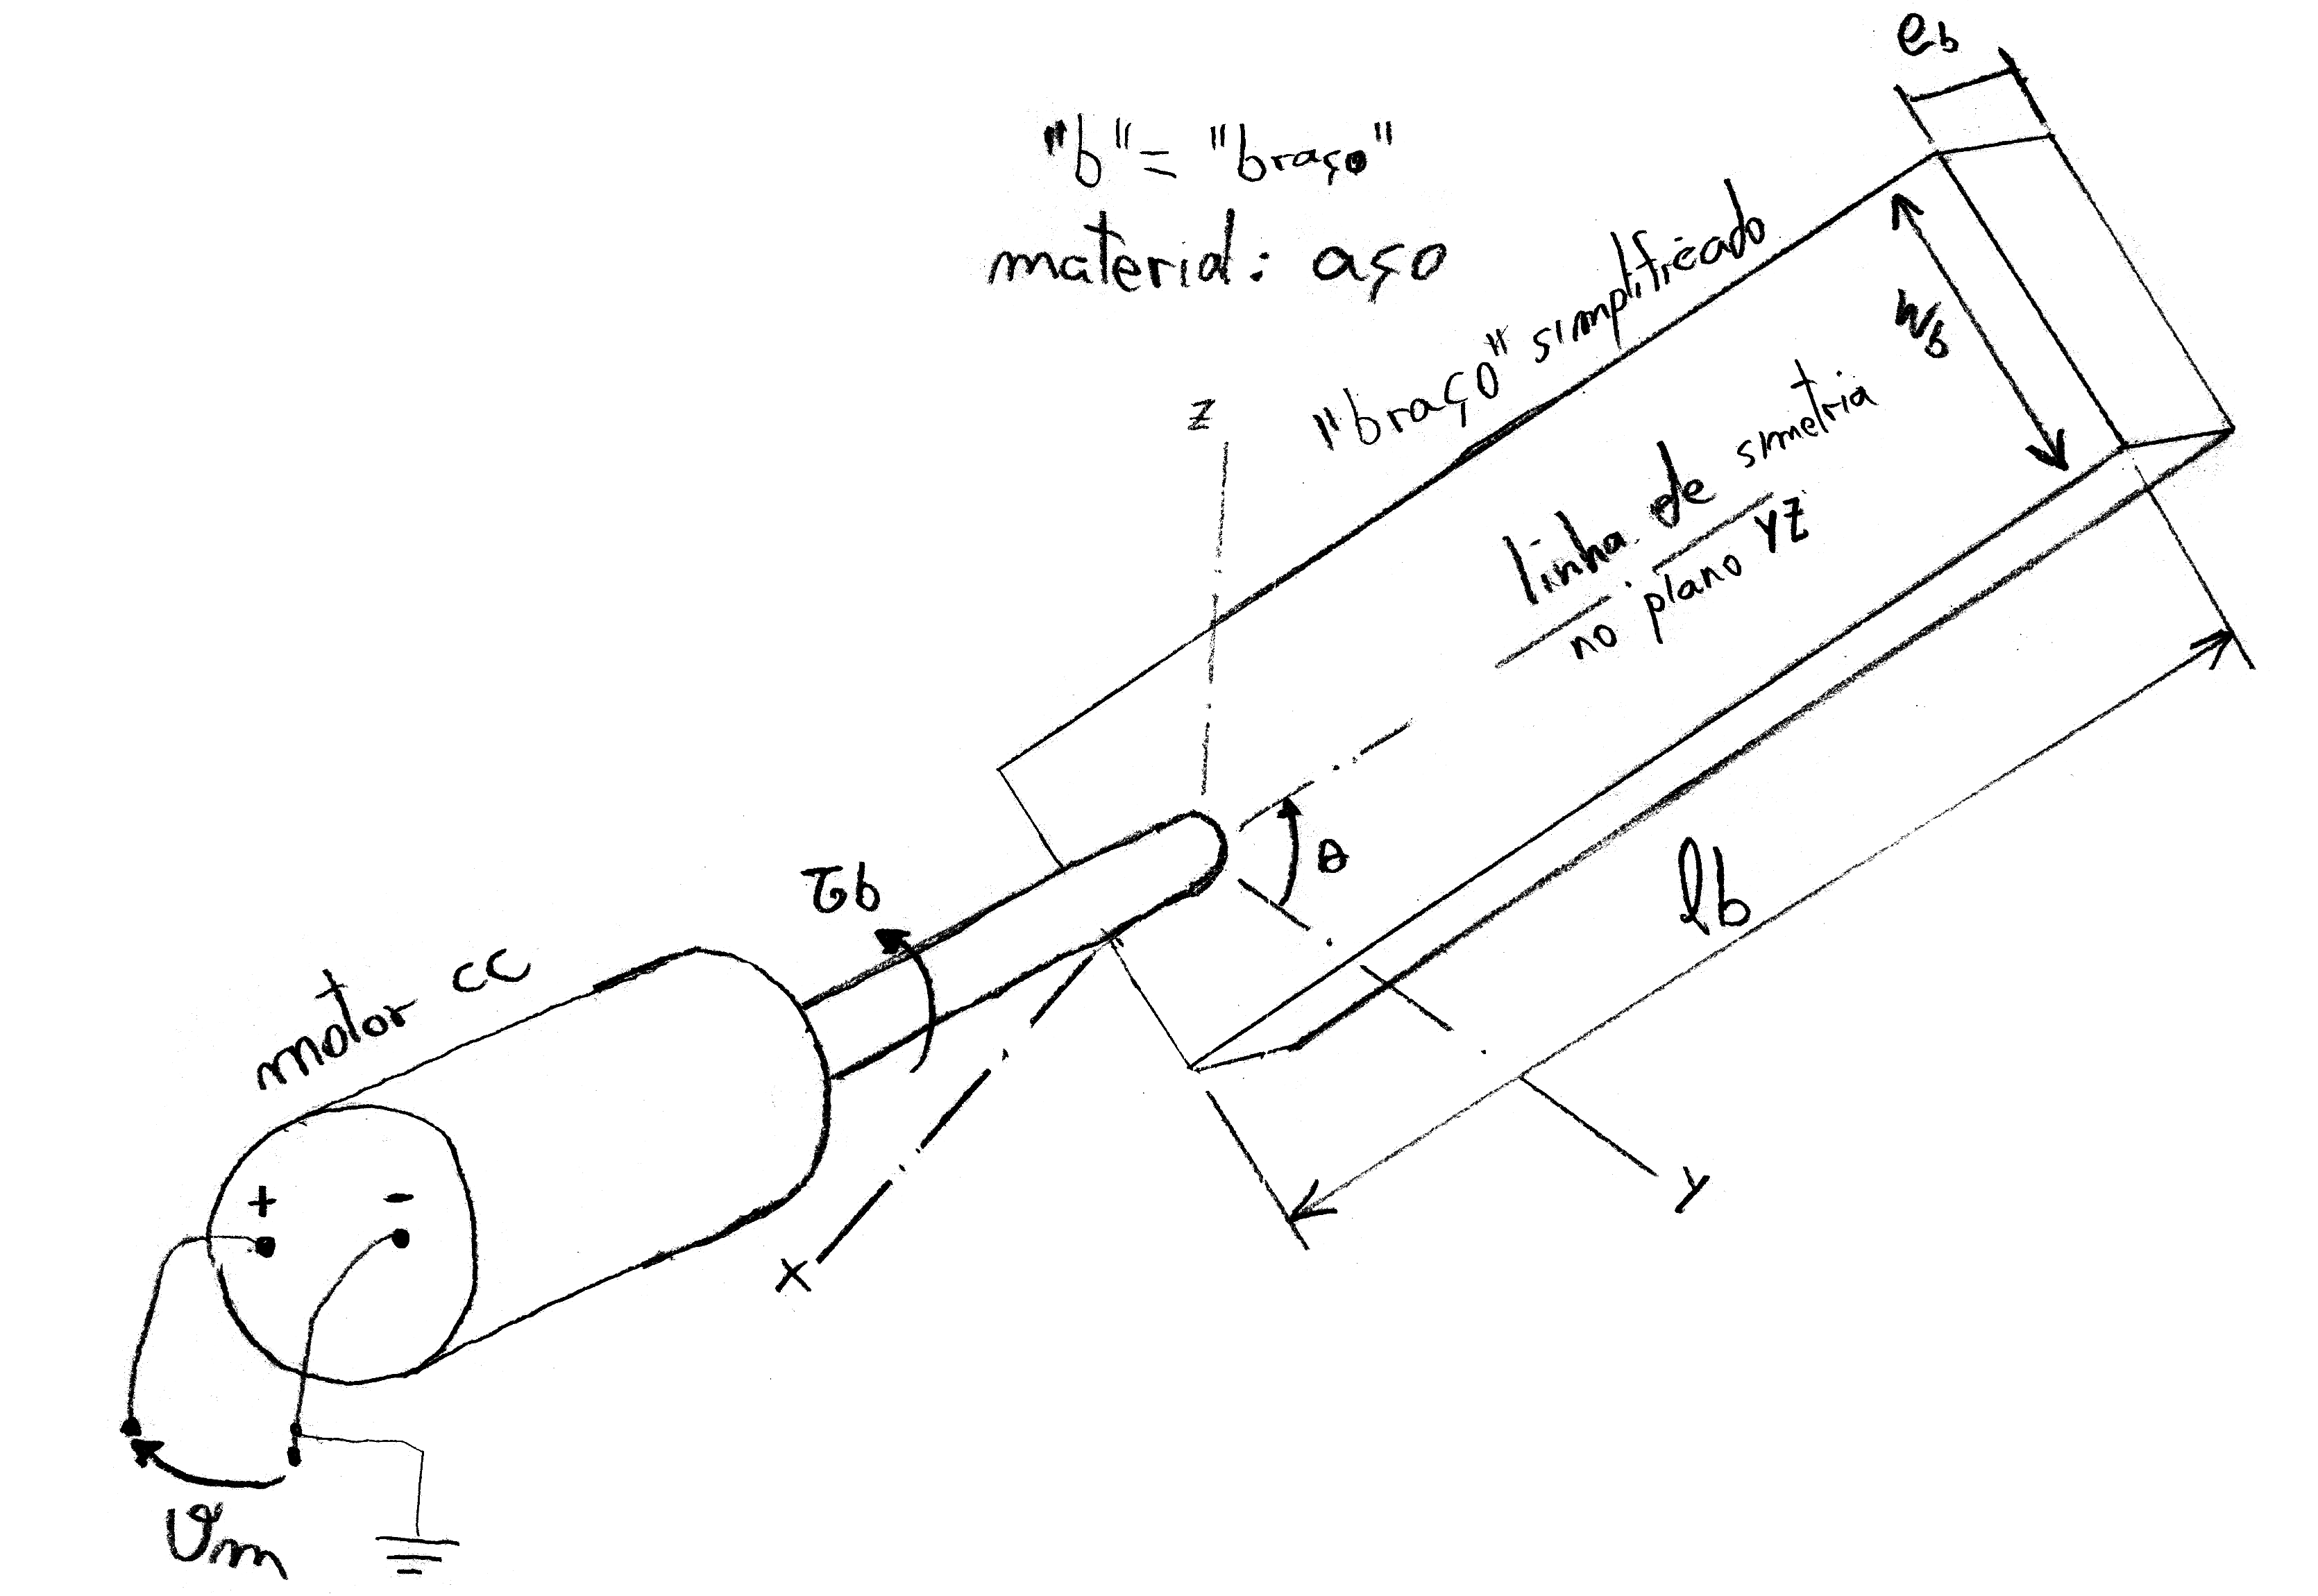
\includegraphics[width=1\textwidth]{motorEBraco.png}
\caption{\label{fig:motorEBraco} Desenho esquemático de um braço simplificado.}
\end{figure}

As principais considerações do modelo que usaremos são as seguintes:

\begin{enumerate}
    \item A barra é uniforme e está livre de qualquer esforço externo (inclusive da gravidade).
    \item O eixo de conexão não possui massa.
    \item O motor possui uma inércia interna concentrada e um engrenamento perfeito de redução. 
    \item O motor é de ímã permanente e sua constante de torque é igual à constante de força eletromotriz. 
    \item Os atritos da carga (a inércia da barra) e interno do motor são do tipo viscoso linear (proporcional à velocidade angular).
\end{enumerate}

Para ver como o sistema foi modelado detalhadamente, clique no link abaixo: \\

\url{} \\ % PREENCHER PREENCHER PREENCHER PREENCHER PREENCHER PREENCHER

O sistema mecânico resulta em uma inércia equivalente $J_{eq}$ e um coeficiente de atrito equivalente $f_{eq}$. Sob $J_{eq}$ é aplicado o torque gerado pelo acoplamento magnético, criando a aceleração angular $\ddot{\theta_b}$, conforme a Equação \ref{eqn:mecanico}. \

O sistema elétrico é composto por uma fonte ideal, uma resistência, uma indutância e uma força eletromotriz; todos em sériem resultando na Equação \ref{eqn:eletrico}. \

O acoplamento eletromecânico é modelado com relações lineares entre o torque e a corrente do circuito ($\tau_m = K_m i_m$) e entre a velocidade de rotação do braço e a força eletromotriz ($e_m = \frac{K_m}{r_e} \dot{\theta_b}$). \\

Equações \ref{eqn:mecanico} e \ref{eqn:eletrico}: 

\begin{equation}\label{eqn:mecanico}
    \tau_m = J_{eq} \ddot{\theta_b} + f_{eq} \dot{\theta_b}
\end{equation}

\begin{equation}\label{eqn:eletrico}
    v_m = R_m i_m + L_m \frac{di_m}{dt} + \frac{K_m}{r_e} \dot{\theta_b}
\end{equation}


% Espaço de Estados ---------------------------------------------------
\section{Espaço de estados}\label{sec-ee}

!ATENÇÃO! A partir daqui até o final da Seção \ref{sec-sislin}}, trata-se de uma explicação simplificada da elaboração matemática do problema. ESTAS PARTES SÃO OPCIONAIS! \
Se você quiser ir direto para o exercício de implementação do método numérico, vá para a Seção de Exercícios (\ref{sec-exer}) Caso você queira entender como o problema foi formulado (altamente recomendado), leia tudo (não é muito).

Definimos um espaço de estados de dimensão três da seguinte maneira:

\begin{equation*}  
    \pmb{\mathrm{x}} 
    =   \begin{bmatrix} 
            \theta_b \\ 
            \dot{\theta_b} \\ 
            i_m
        \end{bmatrix}   
    \implies 
    \pmb{\dot{\mathrm{x}}} 
    =   \begin{bmatrix} 
            \dot{\theta_b}\\ \\ 
            \ddot{\theta_b} \\ \\
            \dfrac{di_m}{dt}
        \end{bmatrix}
\end{equation*}  

A partir das Equações \ref{eqn:mecanico} e \ref{eqn:eletrico}, obtemos a seguinte expressão para o vetor $\pmb{\dot{\mathrm{x}}} $:

\begin{equation*}       
    \pmb{\dot{\mathrm{x}}} 
    =   \begin{bmatrix} 
            \dot{\theta_b} \\ \\ 
            -\dfrac{f_{eq}}{J_{eq}} \dot{\theta_b} + \dfrac{K_m}{J_{eq}} i_m \\ \\
            - \dfrac{K_m}{r_e L_m} \dot{\theta_b} - \dfrac{R_m}{L_m} i_m + \dfrac{1}{L_m} v_m
        \end{bmatrix}
    =   \underbrace{
		\begin{bmatrix} 
            0 &            1            &          0         \\ \\ 
            0 & -\dfrac{f_{eq}}{J_{eq}} & \dfrac{K_m}{J_{eq}} \\ \\
            0 & -\dfrac{K_m}{r_e L_m}   &  -\dfrac{R_m}{L_m}
        \end{bmatrix}
		}_\text{A}
		\underbrace{
        \begin{bmatrix} 
            \theta_b \\ \\ 
            \dot{\theta_b}  \\ \\
            \dfrac{di_m}{dt} 
        \end{bmatrix}
		}_\text{\pmb{\mathrm{x}}}
        +
		\underbrace{
        \begin{bmatrix} 
            0 \\ \\ 
            0 \\ \\
            \dfrac{1}{L_m} 
        \end{bmatrix}
		}_\text{B}
		\underbrace{
        \begin{bmatrix} 
            v_m 
        \end{bmatrix}
		}_\text{\pmb{u}}
\end{equation*}

\\

\begin{equation}\label{eqn:syscont}
    \pmb{\dot{\mathrm{x}}} \, (t) = A \, \pmb{\mathrm{x}} (t)  + B \, \pmb{u}(t) 
\end{equation}

Ou seja, conforme mostra a Equação \ref{eqn:syscont}, obtemos uma expressão para a derivada do espaço de estados com termos lineares que dependem do próprio espaço de estados ($\pmb{\mathrm{x}} = [\theta_b \quad \dot{\theta_b} \quad i_m]^T$) e do vetor de comando ($\pmb{u} = [v_m]$).\\

O vetor comando é o \textit{input} do sistema; isso significa que ele é a única coisa que podemos controlar diretamente - todo o resto apenas reage às mudanças do \textit{input}. Esta equação é continua no tempo, o que exige a resolução de uma equação diferencial ordinária. Porém, podemos discretizar o sistema e obter uma equação diferença.\\

A discretização temporal é feita com intervalos de $T_s$ segundos ("$s$" de "sampling", que significa "amostragem" em inglês). Isso significa que passaremos a analisar o sistema nos em instantes de tempo $t = k \, T_s,$ para $k = 0, 1, ..., K$. \ 
Ou seja:

\begin{equation}\label{eqn:discretização}
    \pmb{\mathrm{x}}(t) = \pmb{\mathrm{x}}(k \, T_s), \quad k = 0, 1, ..., K.
\end{equation}

Desta forma descrevemos o sistema em instantes de tempo discretos e em um intervalo finito. Para simplificar um pouco a escrita, usaremos a seguinte notação: 

\begin{equation}\label{eqn:notação}
    \pmb{\mathrm{x}}(t) = \pmb{\mathrm{x}}(k \, T_s), \quad k = 0, 1, ..., K
\end{equation}

Então:

\begin{equation}\label{eqn:sysdisc}
    \pmb{\mathrm{x}}_{k \, + \, 1} = \mathrm{a} \, \pmb{\mathrm{x}}_k + \mathrm{b} \, \pmb{u}_k
\end{equation}

Usando a formulação discreta, em vez de resolver a Equação \ref{eqn:syscont}, calcularemos os valores numéricos da Equação \ref{eqn:sysdisc} em $k = 0, 1, ..., K$, onde as matriz a e b serão obtidas usando uma função de discretização do MATLAB - as transformações feitas por esta função fogem do escopo desta formulação; para mais informações, consulte a referência da função "c2d" do MATLAB.

\section{Sistema linear}\label{sec-sislin}

Ok, vamos ao que interessa... \\

Conhecemos, por suposição, os valores iniciais de $\theta_b$, $\dot{\theta_b}$ e $i_m$; portanto conhecemos $\pmb{\mathrm{x}}_0$. No instante de tempo $t = K \, T_s$, queremos que $\theta_b = \theta_F$, $\dot{\theta_b} = 0$ e $i_m = 0$. A corrente deve ser nula para que o torque seja nulo ($\tau_m = K_m \, i_m$). \\

Substituindo $k$ por $0$ e $K$ em \ref{eqn:sysdisc} e rearranjando os termos, obtemos: 

\begin{equation}\label{eqn:k0}
    \pmb{\mathrm{x}}_1 - \mathrm{b} \, \pmb{u}_0 = \mathrm{a} \, \pmb{\mathrm{x}}_0,
    \quad
    \text{onde }
        \pmb{\mathrm{x}}_0 = 
        \begin{bmatrix}
            0 \\
            0 \\
            0
        \end{bmatrix}
\end{equation}

\begin{equation}\label{eqn:kK}
    \mathrm{a} \, \pmb{\mathrm{x}}_{K-1} - \mathrm{b} \, \pmb{u}_{K - 1} = - \pmb{\mathrm{x}}_K, 
    \quad
    \text{onde }
        \pmb{\mathrm{x}}_K = 
        \begin{bmatrix}
            \theta_F \\
            0 \\
            0
        \end{bmatrix}
\end{equation}

Fazendo o mesmo para um $k$ genérico tal que $k = 1, ..., K - 1$, temos: 

\begin{equation}\label{eqn:k}
    \pmb{\mathrm{x}}_{k+1} - \mathrm{a} \, \pmb{\mathrm{x}}_k - \mathrm{b} \, \pmb{u}_k = 0, 
    \quad para \, k = 1, ..., K - 1
\end{equation}

Vamos usar as Equações \ref{eqn:k0}, \ref{eqn:kK} e  \ref{eqn:k} para montar um sistema linear onde as incógnitas são $x_1, x_2, \dots, x_{K-1}, x_K$.
\
Neste mesmo sistema linear, também incluiremos equações de restrições quanto aos valores numéricos de $\pmb{u}_k$ usando a equação de um controlador proporcional (perceba que os valores de $\pmb{u}_k$ também são incógnitas). 
\
Usar um controlador proporcional significa que o \textit{input} (tensão de entrada) é proporcional à diferença entre o valor de $\theta_F$, que é o objetivo, e $\theta_k$, que é o valor de $\theta$ nos estados intermediários, conforme a Equação \ref{eqn:ctrlP}:

\begin{equation}\label{eqn:ctrlP}
    \pmb{u}_{k+1} = K_P \, (\theta_F \, - \, \theta_k) 
	\
	OU 
	\
	\pmb{u}_{k+1} + K_P \, \theta_k = K_P \, \theta_F 
    \quad para \, k = 0, 1, ..., K
\end{equation}

Onde $K_P$ é uma constante de proporcionalidade. Não entraremos no detalhe da teoria de controle, mas perceba que, intuitivamente, faz sentido pensar que o sinal de entrada seja maior (ou seja, mais "forte") quanto maior for a distância da posição até o objetivo (ou seja, mais "longe da linha de chegada").
\
Consequentemente, quando o sistema se aproxima do objetivo, o sinal diminui proporcionalmente, fazendo com que o sistema retorne progressivamente a um estado sem movimento.

\\

Assim, podemos transformar o problema em um sistema linear com o seguinte formato:

\begin{equation} \label{eqn:syslin}
\end{equation}

Chamaremos a matriz deste sistema de $M$, o vetor independente de $vet$ e o vetor de variávels de $Sol$ (de "Solução").

\section{Exercício} \label{sec-exer}

O objetivo do exercício é apenas um: implementar uma função em MATLAB que resolva o sistema linear $M \, Sol = vet$. ATENÇÃO: perceba que a matriz $M$ é retangular e tem mais linhas do que colunas.
\
Você pode consultar qualquer material que achar conveniente para encontrar um algoritmo de resolução de sistemas lineares deste tipo. Dica: comece lendo sobre método QR \href{}{aqui}.
\
O código pré-pronto do MATLAB pode ser encontrado neste \href{}{link}. Você deve baixá-lo, abrir o script "MotorDC_PRINCIPAL.m" e executá-lo para ver qual é o resultado esperado.
\
No código, na seção "Solução do sistema linear", a linha "Sol = M\vet;" deve ser posteriormente comentada - esta é a linha que chama o resolvedor de sistemas lineares do MATLAB.
\
Você deve então escrever o código de implementação do método no arquivo "resolveSistema.m", que é uma função do MATLAB cujas entradas são $M$ e $vet$ e a saída é $Sol$.
\
Após isto, basta descomentar a linha "Sol = resolveSistema(M,vet);" do script principal e testar sua função.
\\
Dica: teste a função anteriormente com exemplos mais simples e conhecidos. Quando ele funcionar corretamente, tente usá-lo no script do motor DC.

\bigskip

Envie seu arquivo de código para \textbf{joao.bertoldo@usp.br} com cópia para \textbf{efcosta@icmc.usp.br} com o assunto "Exercício Adicional 3 - xx", onde "xx" é o seu nome.

\bigskip

\centering{\Large{Boa sorte!}}

\end{document}